\documentclass[9pt,a4paper]{ctexart}
\usepackage[margin=1.2cm]{geometry}
\usepackage{graphicx}
\usepackage{hyperref}
\usepackage{enumitem}
\usepackage{titlesec}
\usepackage{array}
\usepackage{booktabs}
\usepackage{amssymb}
\setlength{\parskip}{0.1em}
\setlength{\parindent}{0pt}
\titlespacing{\section}{0pt}{0.2em}{0em}
\titlespacing{\subsection}{0pt}{0.1em}{0em}
\setlist{noitemsep,topsep=0pt,partopsep=0pt,leftmargin=*}
\hypersetup{colorlinks=true,linkcolor=blue,urlcolor=cyan}

\begin{document}

{\centering
{\LARGE\bfseries 塔防游戏 — 面向对象架构设计说明}\\[0.2em]
{\normalsize 2026 夏 · 小学期大作业}\\[-0.5em]
}

\section{项目概述}
基于\texttt{matplotlib FuncAnimation}的塔防游戏：玩家在15$\times$9网格上放置防御塔，
阻止沿路径前进的敌人到达基地。包含\textbf{10波递增难度}、\textbf{3种塔}、\textbf{3种敌人}。
技术栈：\textbf{Python 3} + \textbf{NumPy}（向量计算）+ \textbf{Matplotlib}（实时渲染+事件处理）+
\textbf{Pandas}（战后统计）。运行：\texttt{python main.py}。结构：\texttt{main.py} $\rightarrow$ \texttt{src/}（8模块）$\rightarrow$ \texttt{doc/}。

\section{类层次结构与UML图}
项目共\textbf{11个类}，\textbf{3条继承链}。UML类图（draw.io制作）见图\ref{fig:uml}，
源文件：\texttt{doc/uml\_diagram.drawio}。

\begin{figure}[htbp]
    \centering
    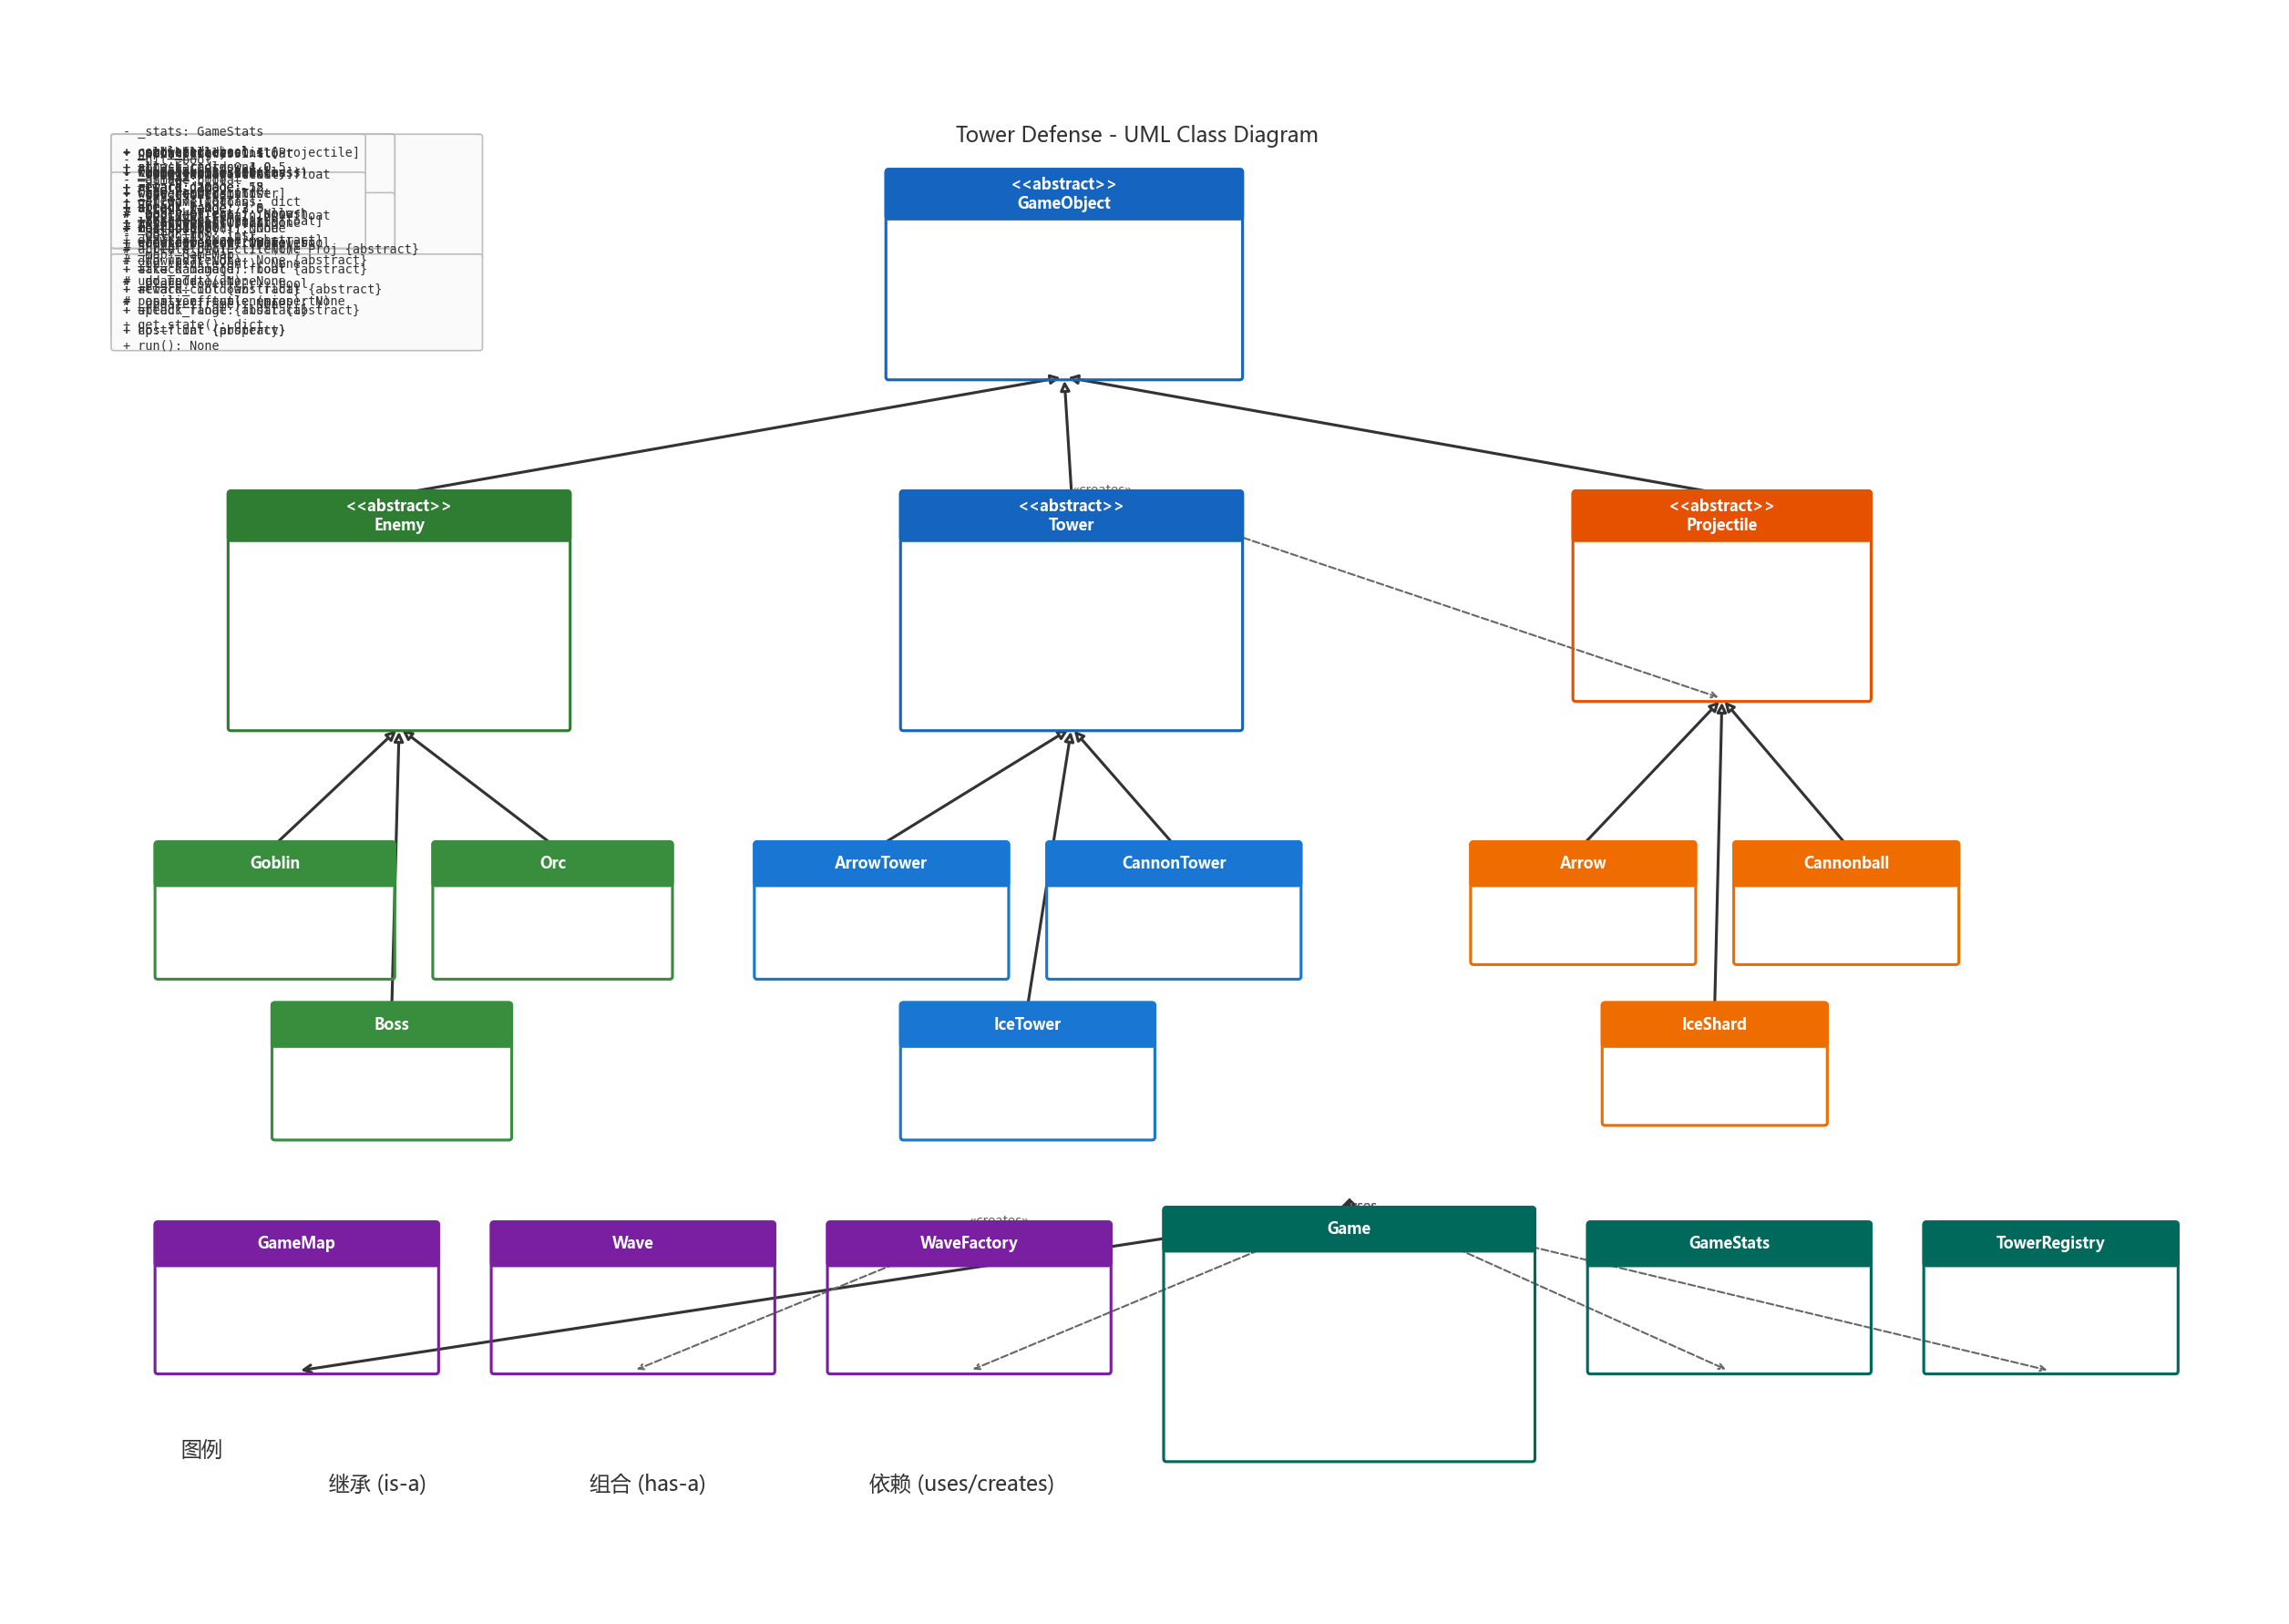
\includegraphics[width=0.85\textwidth,height=0.30\textheight,keepaspectratio]{uml_diagram.png}
    \caption{塔防游戏UML类图（draw.io绘制）}
    \label{fig:uml}
\end{figure}

\subsection*{继承链与辅助类一览}

{\footnotesize\renewcommand{\arraystretch}{0.85}
\begin{tabular}{@{}>{\ttfamily}ll>{\raggedright\arraybackslash}p{5cm}@{}}
\toprule
\rmfamily\textbf{类名} & \textbf{类型} & \textbf{关键成员} \\
\midrule
GameObject & ABC & \_position, \_size, \_alive; \quad update(dt), draw(ax), \_do\_update() \\
\quad Enemy & ABC & hp, speed, reward, slow\_factor;  take\_damage(), apply\_slow() \\
\quad\quad Goblin  & 具体 & HP=60, 速度2.5, 奖励10, 基地伤害1 \\
\quad\quad Orc     & 具体 & HP=180, 速度1.5, 奖励25, 基地伤害2 \\
\quad\quad Boss    & 具体 & HP=600, 速度0.9, 奖励100, 基地伤害5 \\
\quad Tower & ABC & cost, attack\_range, cooldown;  \_create\_projectile(), record\_kill() \\
\quad\quad ArrowTower  & 具体 & 造价50, 射程3.0, 冷却0.5s, 伤害18（单体） \\
\quad\quad CannonTower & 具体 & 造价100, 射程2.5, 冷却1.5s, 伤害55（溅射1.0格） \\
\quad\quad IceTower    & 具体 & 造价75, 射程2.8, 冷却1.0s, 伤害12（减速40\%,2s） \\
\quad Projectile & ABC & target, speed, damage;  \_apply\_effect() \\
\quad\quad Arrow / Cannonball / IceShard & 具体 & 单伤18 | 溅射55(半伤) | 减速12 \\
\midrule
GameMap & 工具 & 15$\times$9网格, waypoints, path\_cells;  can\_place\_tower(), cell\_center() \\
Wave   & 数据 & wave\_number, spawn\_events;  get\_spawns(), completed \\
WaveFactory & 工厂 & \_configs;  create\_wave(n), total\_waves()（注册表模式） \\
TowerRegistry & 工厂 & \_registry;  create(name,col,row), list\_types()（简单工厂） \\
Game   & 主控 & \_map, \_gold, \_base\_hp, 实体列表;  run(), \_update(), \_place\_tower() \\
GameStats & 统计 & wave\_records, kill\_events;  show\_report()（Pandas+4图表） \\
\bottomrule
\end{tabular}
}

\section{类间关系}
\begin{itemize}
    \item \textbf{继承：} Goblin/Orc/Boss $\rightarrow$ Enemy $\rightarrow$ GameObject（空心三角实线）；
          ArrowTower/CannonTower/IceTower $\rightarrow$ Tower $\rightarrow$ GameObject；
          Arrow/Cannonball/IceShard $\rightarrow$ Projectile $\rightarrow$ GameObject
    \item \textbf{组合：} Game $\blacklozenge\rightarrow$ GameMap（实心菱形，同生命周期）
    \item \textbf{依赖：} Tower $\rightarrow$ Projectile（工厂方法创建，虚线箭头）；
          WaveFactory $\rightarrow$ Wave；Game $\rightarrow$ WaveFactory / GameStats / TowerRegistry
\end{itemize}

\section{设计模式}
\textbf{策略模式：} Tower定义统一攻击接口，三种子类覆写属性实现不同策略。
主循环通过\texttt{for t in towers: t.update(...)}多态调用（对标Day6 Grader）。

\textbf{模板方法：} GameObject.update()检查存活后调用\_do\_update()，子类只覆写钩子方法。

\textbf{工厂模式：} WaveFactory注册表管理10波配置；TowerRegistry字符串→类映射（对标Day6 SolverFactory）。

\textbf{组合优于继承：} Game组合GameMap+实体列表+Stats；新增敌人只需注册（开闭原则）。

\section{GitHub仓库}
\url{https://github.com/TYJ-xy/tower-defense-oop}

\end{document}
